\section{RET - Reaktanz-Eintore}
\subsection{Reaktanzen}
	\begin{tabular}{ll ll}
		\parbox{4cm}{
		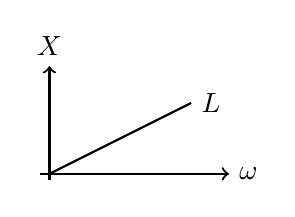
\begin{tikzpicture}[scale=0.6, yscale=0.6, thick]
	%Koordinatensystem
	\draw[->] (-0.2,0) -- +(right:4) node[right] {$\omega$};
	\draw[->] (0,-0.2) -- +(north:4) node[above] {$X$};
	\draw (0,0) -- (3,2.5) node[right] {$L$};
\end{tikzpicture}



			%\includegraphics[width=3.5cm]{./bilder/Induktivitaet}
			}
			& \parbox{5cm}{
				\textbf{Induktivität} \\
				$\underline{Z}=j\omega L \qquad X=\omega L$\\
				$B=-\frac{1}{\omega L}$\\
				Nullstelle: $\lim\limits_{\omega \rightarrow 0} X(\omega) = 0$ \\
				Polstelle: $\lim\limits_{\omega \rightarrow \infty} X(\omega) = \infty$ \\
			}
			
			& \parbox{4cm}{
			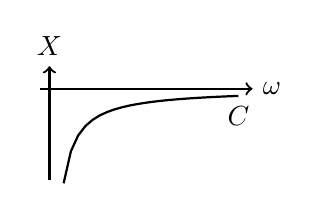
\begin{tikzpicture}[scale=0.6, yscale=0.6, thick]
	%Koordinatensystem
	\draw[->] (-0.2,0) -- +(right:4.5) node[right] {$\omega$};
	\draw[->] (0,-3.2) -- +(north:4) node[above] {$X$};
	\draw plot[domain=0.3:4] (\x,{-1/(\x)})
	node[below] {$C$};
\end{tikzpicture}



			%\includegraphics[width=3.5cm]{./bilder/Kapazitaet}
			}
			& \parbox{5cm}{
				\textbf{Kapazität} \\
				$\underline{Z}=\frac{1}{j\omega C}=-\frac{j}{\omega C} \qquad X=-\frac{1}{\omega C}$\\
				$B=\omega C$ \\
				Nullstelle: $\lim\limits_{\omega \rightarrow \infty} X(\omega) = 0$ \\
				Polstelle: $\lim\limits_{\omega \rightarrow 0} X(\omega) = -\infty$ \\
			}
	\end{tabular}

\begin{multicols}{2}
	
\subsection{Vorgehen bei Netzwerkanalyse}
	\begin{enumerate}{\setlength{\itemsep}{0cm}\setlength{\parsep}{0cm} \setlength{\topsep}{0cm}}
      \item Schaltung übersichtlich aufzeichenen und den Startpunkt der Addition bestimmen
      \item Frequenzverlauf der Reaktanz finden durch fortgeschrittene Addition und Inversion
      \item Inversion: $B(\omega)=-\frac{1}{X(\omega)}$ ; $Polstelle \Longleftrightarrow Nullstelle$
      \item Die so entstandenen Pole und Nullstellen, ausser 0 und $\infty$ sind die Resonanzfrequenzen des RET
    \end{enumerate}
    
    
\subsection{RET Eigenschaften}
	\begin{itemize}
		\item \textbf{Zähler/Nenner-Potenz} - Der Zahler hat entweder/oder gerade/ungerade Potenzen, wohin gegen der Nenner ungerade/gerade Potenzen von $j\omega$ besitzt
		\item Den Polynomen fehlen keine Koeffizienten!
		\item \textbf{Anzahl Elemente} - Anzahl nicht-negativen und endlichen Polen/Nullstellen entspricht minimale Anzahl Elemente
	\end{itemize}
	
\end{multicols}	

\renewcommand{\arraystretch}{2}
\begin{sidewaystable}
\subsection{RET-Typen}
\begin{tabular}{|p{1.7cm}|l|l|l|l|l|p{1.5cm}|p{1.9cm}|l|}
\hline
	\textbf{Symbol} &
	\textbf{Typ} &
	\textbf{Reaktanz} &
	\textbf{Impedanzfunktion} &
	\multicolumn{2}{|c|}{\textbf{Eigenschaften}} &
	$\bf \boldsymbol\omega = 0$ \newline $\bf \boldsymbol\omega \rightarrow \boldsymbol\infty$ &
	Zähler (n) &	Nenner (m) 
	\\
\hline
	\parbox[c][1.5cm]{1.2cm}{\begin{circuitikz}[scale=2, european, american inductors, yscale=0.4]
\ctikzset{bipoles/length=0.5cm}
\draw (0,0)
	to[L, *-*] (0.7cm,0)
	;	
\end{circuitikz}
} &
	L-Typ &
	\parbox[c][3cm]{5.3cm}{\usepgflibrary{shapes.misc}
\begin{tikzpicture}[smooth, xscale=0.5, yscale=0.5]
% Achsen
\draw[->, thick] (-0.2,0) -- +(8,0) node[right] {$\omega$}; % Horizontal
\draw[->, thick] (0,-2) -- +(0,4) node[above] {$X(\omega)$}; % Vertikal

% Plots
\draw[color=green!70!black, thick] plot[domain=0:1.1] (\x,{tan(\x r)}); % Erster Tan
\draw[color=green!70!black, thick] plot[domain=2.01:4.23] (\x,{tan(\x r)}); % zweiter Tan
\draw[color=green!70!black, thick] plot[domain=4.91:8] (\x,{ (0.25 * \x) -1/(\x -4.6) }); % letzte kurve

% Poolstellen
\draw[dashed, thick, draw=red] (1.57,-2.1) -- +(0,4.2); % Poolstelle 1
\draw[dashed, thick, draw=red] (4.71,-2.1) -- +(0,4.2); % Poolstelle 2
\node[cross out, draw=red, thick] (wr1) at (1.57,0) {};
\node[cross out, draw=red, thick] at (4.71,0) {};


\draw[dashed] plot[domain=0:8] (\x, { 0.25 * \x});
\node (wL) at (6.1,2.4) {$\omega L_\infty$};

% Nullstellen
\node[rounded rectangle, draw=blue, thick] at(0,0) {};
\node[rounded rectangle, draw=blue, thick] at(3.141,0) {};
\node[rounded rectangle, draw=blue, thick] at(5.35,0) {};
\end{tikzpicture}}&
	\begin{tabular}{cl}
	 $ \underline{Z}(p)$ & $ =p\frac{a_np^{n-1}+ \ldots +a_1}{b_mp^m+ \ldots b_0}$
	 \\ 
	 & $=\frac{j\omega
	L_{\infty}[(j\omega)^2+\omega_3^2][\ldots]}{[(j\omega)^2+\omega_2^2][\ldots]}$
	\end{tabular} &
	L-Kreis &
	L-TB &
	Null \newline Pol &
	ungerade & $m=n-1$
	\\
\hline
	\parbox[c][1.5cm]{1.2cm}{\input{tikzPictures/RET/C.tex}} &
	C-Typ &
	\parbox[c][3cm]{5.3cm}{\usepgflibrary{shapes.misc}
\begin{tikzpicture}[smooth, xscale=0.5, yscale=0.5]
% Achsen
\draw[->, thick] (-0.2,0) -- +(9,0) node[right] {$\omega$}; % Horizontal
\draw[->, thick] (0,-2) -- +(0,4) node[above] {$X(\omega)$}; % Vertikal

% Plots
\draw[color=green!70!black, thick] plot[domain=0.45:2.68] (\x,{tan((\x -1.57) r)}); % Erster Tan
\draw[color=green!70!black, thick] plot[domain=3.58:5.8] (\x,{tan((\x -1.57) r)}); % zweiter Tan
\draw[color=green!70!black, thick] plot[domain=6.78:8.6] (\x,{ ((0.25 * \x) -1/(\x -6.3)) -2 }); % letzte kurve

% Poolstellen
\draw[dashed, thick, draw=red] (3.14,-2.1) -- +(0,4.2); % Poolstelle 1
\draw[dashed, thick, draw=red] (6.28,-2.1) -- +(0,4.2); % Poolstelle 2
\node[cross out, draw=red, thick] (wr1) at (3.14,0) {};
\node[cross out, draw=red, thick] at (6.28,0) {};
\node[cross out, draw=red, thick] at (0,0) {};


\draw[dashed] plot[domain=5:8.7] (\x, { (-1 /(0.04 * \x)) + 2.7 });
\begin{scope}[transform shape, scale=1.7]
	\node (wL) at (2.85,-0.7) {$- \frac{1}{\omega C_\infty}$};
\end{scope}

% Nullstellen
\node[rounded rectangle, draw=blue, thick] at(1.57,0) {};
\node[rounded rectangle, draw=blue, thick] at(4.71,0) {};
\end{tikzpicture}} &
	\begin{tabular}{cl}
	  $\underline{Z}(p)$&
	  $=\frac{1}{p}\frac{a_np^{n}+ \ldots +a_0}{b_mp^{m-1}+\ldots	b_1} $ \\
	  & $=\frac{[(j\omega)^2+\omega_2^2][\ldots]}{j\omega
	  C_{\infty}[(j\omega)^2+\omega_3^2][\ldots]}$	  
	\end{tabular} &
	C-Kreis &	
	C-TB &
	Pol \newline Null &
	gerade & $m=n+1$
	\\
\hline
	\parbox[c][1.5cm]{1.2cm}{\begin{circuitikz}[scale=2, european, american inductors, yscale=0.3]
\ctikzset{bipoles/length=0.5cm}
\draw (0,0)
	to[C, *-] (0.35cm,0)
	to[L, -*] (0.7cm,0)
	;	
\end{circuitikz}
} &
	S-Typ &
	\parbox[c][3cm]{5.3cm}{\usepgflibrary{shapes.misc}
\begin{tikzpicture}[smooth, xscale=0.5, yscale=0.5]
% Achsen
\draw[->, thick] (-0.2,0) -- +(9,0) node[right] {$\omega$}; % Horizontal
\draw[->, thick] (0,-2) -- +(0,4) node[above] {$X(\omega)$}; % Vertikal

% Plots
\draw[color=green!70!black, thick] plot[domain=0.45:2.68] (\x,{tan((\x -1.57) r)}); % Erster Tan
\draw[color=green!70!black, thick] plot[domain=3.58:5.8] (\x,{tan((\x -1.57) r)}); % zweiter Tan
\draw[color=green!70!black, thick] plot[domain=7.05:9.5] (\x,{ (0.25 * \x) -1/(\x -6.8) }); % letzte kurve

% Poolstellen
\draw[dashed, thick, draw=red] (3.14,-2.1) -- +(0,4.2); % Poolstelle 1
\draw[dashed, thick, draw=red] (6.28,-2.1) -- +(0,4.2); % Poolstelle 2
\node[cross out, draw=red, thick] (wr1) at (3.14,0) {};
\node[cross out, draw=red, thick] at (6.28,0) {};
\node[cross out, draw=red, thick] at (0,0) {};


\draw[dashed] plot[domain=0.55:3.5] (\x, { (-1 /(0.8* \x))});
\begin{scope}[transform shape, scale=1.7]
	\node (wL) at (1.2,-0.9) {$- \frac{1}{\omega C_0}$};
\end{scope}

\draw[dashed] plot[domain=0:9.6] (\x, { 0.25 * \x});
\node (wL) at (7.5,2.5) {$\omega L_\infty$};

% Nullstellen
\node[rounded rectangle, draw=blue, thick] at(1.57,0) {};
\node[rounded rectangle, draw=blue, thick] at(4.71,0) {};
\node[rounded rectangle, draw=blue, thick] at(7.34,0) {};
\end{tikzpicture}} &
	\begin{tabular}{cl}
	  $\underline{Z}(p)$&
	  $=\frac{1}{p}\frac{a_np^{n}+\ldots+a_0}{b_mp^{m-1}+\ldots
	  b_1}$\\
	  &
	  $=\frac{[L_{\infty}(j\omega)^2+\omega_2^2][(j\omega)^2+\omega_4^2][\ldots]}{j\omega[(j\omega)^2+\omega_3^2]\ldots]}$
	\end{tabular} &
	C-TB &
	L-TB &
	Pol \newline Pol &
	gerade & $m=n-1$
	\\
\hline
	\parbox[c][1.5cm]{1.2cm}{\begin{circuitikz}[scale=2, european, american inductors, yscale=0.3]
\ctikzset{bipoles/length=0.5cm}
\draw (0,0)
	to[short, *-] (0.1cm,0)
	(0.1cm,0.5) to[short] (0.1cm,-0.5)
	(0.1cm,0.5) to [L] (0.6cm,0.5)
	(0.1cm,-0.5) to [C] (0.6cm,-0.5)
	(0.6cm,0.5) to [short] (0.6cm,-0.5)
	(0.6cm,0) to [short, -*] (0.7cm,0)
	;	
\end{circuitikz}
} &
	P-Typ &
	\parbox[c][3cm]{5.3cm}{\usepgflibrary{shapes.misc}
\begin{tikzpicture}[smooth, xscale=0.5, yscale=0.5]
% Achsen
\draw[->, thick] (-0.2,0) -- +(9,0) node[right] {$\omega$}; % Horizontal
\draw[->, thick] (0,-2) -- +(0,4) node[above] {$X(\omega)$}; % Vertikal

% Plots
\draw[color=green!70!black, thick] plot[domain=0.01:0.9] (\x, {tan( (\x *1.2) r )        }); % Erster Tan
\draw[color=green!70!black, thick] plot[domain=1.3:3.15] (\x,    {tan( (\x*1.2 -2.7) r)    }); % Erster Tan
\draw[color=green!70!black, thick] plot[domain=3.9:5.75] (\x,  {tan( (\x*1.2 -2.7) r)  }); % zweiter Tan
\draw[color=green!70!black, thick] plot[domain=6.5:8.6] (\x,  { ((0.25 * \x) -1/(\x -6)) -2 }); % letzte kurve

% Poolstellen
\draw[dashed, thick, draw=red] (1,-2.1) -- +(0,4.2); % Poolstelle 1
\node[cross out, draw=red, thick] at (1,0) {};

\draw[dashed, thick, draw=red] (3.4,-2.1) -- +(0,4.2); % Poolstelle 2
\node[cross out, draw=red, thick] at (3.4,0) {};

\draw[dashed, thick, draw=red] (6,-2.1) -- +(0,4.2); % Poolstelle 3
\node[cross out, draw=red, thick] at (6,0) {};

%\node[cross out, draw=red, thick] at (0,0) {};


\draw[dashed] plot[domain=5:8.7] (\x, { (-1 /(0.035 * \x)) + 3.2 });
\node (wC) at (7.5,2) {$- \frac{1}{\omega C_\infty}$};
\draw[->, thick] (7.5,1.2) -- +(-0.5,-1.8);

\draw[dashed] plot[domain=0:2] (\x,{\x});
\node at (2.2,2.4) {$\omega L_0$};


% Nullstellen
\node[rounded rectangle, draw=blue, thick] at(0,0) {};
\node[rounded rectangle, draw=blue, thick] at(2.25,0) {};
\node[rounded rectangle, draw=blue, thick] at(4.86,0) {};
\end{tikzpicture}} &
	\begin{tabular}{cl}
	  $\underline{Z}(p)$&
	  $=p\frac{a_np^{n-1}+\ldots +a_1}{b_mp^m+\ldots b_0}$ \\
	  & $=\frac{j\omega[(j\omega)^2+\omega_3^2][\ldots]}{C_{\infty}[(j\omega)^2+\omega_2^2][(j\omega)^2+\omega_4^2]\ldots]}$
	\end{tabular} &
	C-Kreis & L-Kreis &
	Null \newline Null &
	ungerade & $m=n+1$
	\\
\hline
\end{tabular}
\caption[Bestimmung des RET-Typ]{Bestimmung des RET-Typ. Die Bezeichnungen
Klemmentrennbündel und Klemmenkreis wurden abgekürzt zu TB und Kreis. Die
Reaktanzdiagramme sind keinenfalls Masstäblich!}
\label{tab:RETTyp}


\subsection{Äquivalenz}
	\begin{enumerate}[itemsep=1ex, nosep]
		\item Gegebenes RET übersichtlich aufzeichnen
		\item Ins RET zusätzliche L- bzw. C-Elemente einfügen, dass C- bzw. L-Kreise oder C- bzw. L-Trennbündel entstehen.
		\item Durch Weglassen / Kurzschliessen von alten RET-Elementen das erweitere RET auf ein MRET zurückführen.
		\item Impedanzfunktion des alten RET und des MRET berechnen und die unbekannten MRET-Elemente durch Koeffizientenvergleich bestimmen.
	\end{enumerate}

\end{sidewaystable}
\renewcommand{\arraystretch}{\arraystretchOriginal}		

\subsection{Minimalreaktanzeintor (MRET)}
	%RET in MRET wandeln:\\
	\begin{enumerate}[itemsep=1ex, nosep]
      \item Netzwerk übersichtlich aufzeichnen 
      \item Tor offen; Kreise suchen die nur L oder C enthalten; Ein
      Element des Kreises weglassen, es darf aber kein anderer Zweig stromlos werden. 
      \item Tor kurzgeschlossen; Trennbündel suchen(Knoten, oder Element an denen nur
      L oder C liegen); Ein Element kurzschliessen, dabei darf kein anderes Element kurzgeschlossen werden.
      \item Die verbleibenden Elemente im MRET haben nicht mehr die
      gleichen Grössen und müssen neu berechnet werden.
    \end{enumerate}
	
	Anzahl Elemente entspricht höchster Potenzfunktion $\underline{Z}(p)$
	
\subsection{RET-Synthese}
\begin{multicols}{2}
\subsubsection{Mittels Partialbruchzerlegung}
	\begin{enumerate}
	  \item $\underline{F}(p)=\frac{2p^6+22p^4+68p^2+48}{3p^5+21p^3+30p}$
	  \item $\underline{F}(p)$ ausdividieren, falls Zählergrad $>$ Nennergrad
	  \item Nenner des echten Bruches zerlegen und Ansatz bilden
	  $(\frac{2}{3}p+)
	  \quad\frac{8p^4+48p^2+48}{3p^5+21p^3+30p}=\frac{A}{3p}+\frac{Bp}{p^2+2}+\frac{Cp}{p^2+5}$
		\item Erweitern und Koeffizienten bestimmen\newline $A=\frac{24}{5} \qquad
		B=\frac{8}{9} \qquad C=\frac{8}{45}$
		\item Koeffizienten einsetzen\\
		$\underline{F}(p)=\frac{2}{3}p+\frac{1}{\frac{15}{24}p}+\frac{1}{\frac{9}{8}p+\frac{1}{\frac{4}{9}p}}+\frac{1}{\frac{45}{8}p+\frac{1}{\frac{8}{255}p}}$
		\item Schaltung aufzeichnen:\\
			Impedanzfunktion $\underline{Z}(p)$\\
			\hspace*{0.5cm}\scalebox{0.6}{\begin{circuitikz}[scale=1.5, european, american inductors]
\ctikzset{bipoles/length=1.0cm}
\draw (0,0)
	to [L = $2/3H$, *-] (1,0)
	to [C = $15/24F$, -*] (2,0);
\draw (2,0.5) -- (2,-0.5);
\draw (2,0.5) to [L = $4/9H$] (3,0.5);
\draw (2,-0.5) to [C = $9/8F$] (3,-0.5);
\draw (3,0.5) -- (3,-0.5);
\draw (3,0) to [short, *-*] (3.5,0);
\draw (3.5,0.5) -- (3.5,-0.5);
\draw (3.5,0.5) to [L = $8/225H$] (4.5,0.5);
\draw (3.5,-0.5) to [C = $45/8F$] (4.5,-0.5);
\draw (4.5,0.5) -- (4.5,-0.5);
\draw (4.5,0) to [short, *-*] (5,0);
	;	
\end{circuitikz}}\\
			Admittanzfunktion $\underline{Y}(p)$\\
			\hspace*{0.5cm}\scalebox{0.55}{\begin{circuitikz}[scale=2, european, american inductors]
\ctikzset{bipoles/length=1.2cm}
\draw (0,0) to [short, *-] (4,0);
\draw (0,-2) to [short, *-] (4,-2);
\draw (1,0) to [C = $2/3F$] (1,-2);
\draw (2,0) to [L = $15/24H$] (2,-2);
\draw (3,0) to [L = $9/8H$] (3,-1) to [C = $4/9F$] (3,-2);
\draw (4,0) to [L = $45/8H$] (4,-1) to [C = $8/225F$] (4,-2);	
\end{circuitikz}}	  
	\end{enumerate}
	
\subsubsection{Mittels Kettenbruchzerlegung}
1. Art: Zählergrad $>$ Nennergrad, sonst invertieren\\
2. Art: Polynom nach kleinster Potenz ordnen. Falls Pol bei p=0 $\Rightarrow$ nicht
invertieren, ansonsten invertieren
\begin{enumerate}
	\item $\underline{F}(p)=\frac{2p^6+22p^4+68p^2+48}{3p^5+21p^3+30p}$
	\item $\underline{F}(p)$ ausdividieren $=\frac{2}{3}p+\frac{8p^4+48p^2+48}{3p^5+21p^3+30p}$
	\item Kehrwert des Restes nochmals ausdividieren
	$\frac{2}{3}p+\frac{1}{\frac{3p^5+21p^3+30p}{8p^4+48p^2+48}}=\frac{2}{3}p+\frac{1}{\frac{3}{8}p+\frac{3p^3+12p}{8p^4+48p^2+48}}$
	\item Schritt zwei wiederholen bis kein Rest mehr vorhanden ist
	$\underline{F}(P)=\frac{2}{3}p+\frac{1}{\frac{3}{8}p+\frac{1}{\frac{8}{3}p+\frac{1}{\frac{3}{16}p+\frac{1}{\frac{16}{3}p+\frac{1}{\frac{1}{16}p}}}}}$
	\item Schaltung aufzeichnen  (bei 2. Art L und C vertauschen):\\
		Impedanzfunktion $\underline{Z}(p)$\\
		\hspace*{0.5cm}\scalebox{0.6}{\begin{circuitikz}[scale=1.5, european, american inductors]
\ctikzset{bipoles/length=1.0cm}
\draw (0,0) to [L = $2/3H$, *-] (1,0)
						to [L = $8/3H$] (2,0)
						to [L = $16/3H$] (3,0)
						to [C = $1/16F$] (3,-1)
						to [short, -*] (0,-1);
\draw (1,0) to [C = $3/8F$, *-*] (1,-1);
\draw (2,0)	to [C = $3/16F$, *-*] (2,-1);
\end{circuitikz}}\\
		Admittanzfunktion $\underline{Y}(p)$\\
		\hspace*{0.5cm}\scalebox{0.6}{\begin{circuitikz}[scale=1.8, european, american inductors]
\ctikzset{bipoles/length=1.2cm}
\draw (-0.5,0) to [short, *-] (0,0)
			to [L = $3/8H$] (1,0)
			to [L = $3/16H$] (2,0)
			to [L = $1/16H$] (3,0)
			to [short] (3,-1)
			to [short, -*] (-0.5,-1);
\draw (0,0) to [C = $2/3F$, *-*] (0,-1);
\draw (1,0) to [C = $8/3F$, *-*] (1,-1);
\draw (2,0) to [C = $16/3F$, *-*] (2,-1);
\end{circuitikz}}\\
\end{enumerate}

\end{multicols}


